% Timing model: what each reported quantity covers.
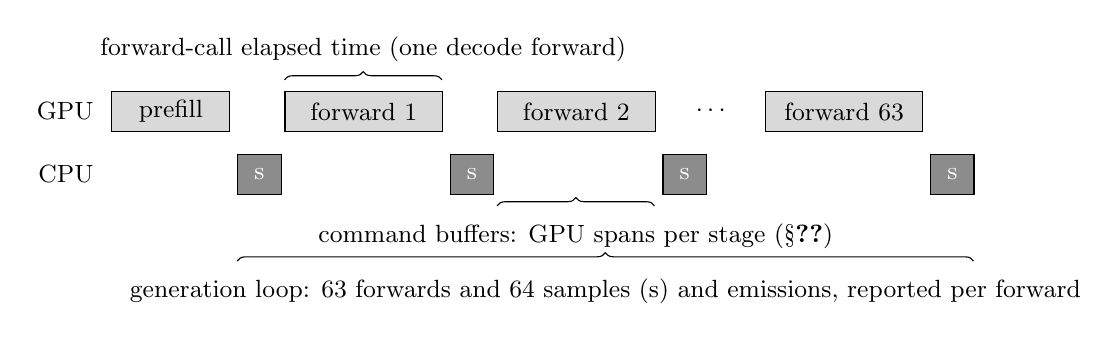
\begin{tikzpicture}[x=1cm,y=1cm,font=\small,
  gpu/.style={draw,fill=black!15,minimum height=0.5cm,inner sep=2pt},
  cpu/.style={draw,fill=black!45,minimum height=0.5cm,inner sep=2pt},
  brace/.style={decorate,decoration={brace,amplitude=3pt}}]
  \node[anchor=east] at (-0.1,1.0) {GPU};
  \node[gpu,minimum width=1.5cm,anchor=west] (pf) at (0,1.0) {prefill};
  \node[gpu,minimum width=2.0cm,anchor=west] (f1) at (2.2,1.0) {forward 1};
  \node[gpu,minimum width=2.0cm,anchor=west] (f2) at (4.9,1.0) {forward 2};
  \node[anchor=west] at (7.3,1.0) {$\cdots$};
  \node[gpu,minimum width=2.0cm,anchor=west] (f63) at (8.3,1.0) {forward 63};
  \node[anchor=east] at (-0.1,0.2) {CPU};
  \node[cpu,minimum width=0.55cm,anchor=west] (s0) at (1.6,0.2) {\textcolor{white}{s}};
  \node[cpu,minimum width=0.55cm,anchor=west] (s1) at (4.3,0.2) {\textcolor{white}{s}};
  \node[cpu,minimum width=0.55cm,anchor=west] (s2) at (7.0,0.2) {\textcolor{white}{s}};
  \node[cpu,minimum width=0.55cm,anchor=west] (s63) at (10.4,0.2) {\textcolor{white}{s}};
  \draw[brace] (2.2,1.4) -- (4.2,1.4) node[midway,above=3pt] {forward-call elapsed time (one decode forward)};
  \draw[brace] (4.9,-0.2) -- (6.9,-0.2) node[midway,below=3pt] {command buffers: GPU spans per stage (\S\ref{sec:method})};
  \draw[brace] (1.6,-0.9) -- (10.95,-0.9) node[midway,below=3pt] {generation loop: 63 forwards and 64 samples (s) and emissions, reported per forward};
\end{tikzpicture}